\section{Methodology and Dataset}
\label{sec:Methodology}

We used \platname to characterize mobile Internet traffic, specifically, we detail the impact of mobile applications, access technology, and operating systems on mobile Internet traffic.

Our analysis methodology included controlled experiments to detail the behavior of specific applications and OS services, and a 7-month long IRB approved measurement study to characterize mobile Internet traffic in the \emph{in the wild}.

\subsection{Controlled Experiments}

For our controlled experiments, we ran the latest versions of Android (Ice Cream Sandwich 4.0, and Jelly-bean 4.2) and iOS 6 respectively on our Android and iOS devices. 
We analyze the behavior of OS services and the default applications by first performing a factory reset on these devices, and installing the \platname credentials on this device.
We then test Android and iOS applications by installing the application, interacting with the application for a few minutes, and finally uninstalling the  application. 
During our controlled experiment we use SSL-Bumping to study the behavior of SSL traffic from these applications. 

Our first experiment included manual testing of the top 100 most popular free Android apps from the \emph{Google Play} store and \tbd{} iOS applications from the iOS App store.
During this experiment, for each application, we enter user credentials for accounts like Facebook and Twitter, and toy with the app for \tbd{} minutes. 

For our second experiment we performed fully-automated tests on 1003 Android applications from a free, third-party Android market.
We perform this test because Android devices can install \emph{Third-party applications} that are not available on the \emph{Google Play} store.
A consequence of this freedom is that numerous third-party app markets are available on the web whose applications have not received research attention.
For our automation we used adb Android command shell to install each app, enable \platname, and start the app.
We then used Monkey, an adb stress tool, to perform a series of 10,000 actions which includes random swipes, touches, and text entries.
We then used adb to uninstall the application and reboot the device to forcibly end any lingering connections.

The results of our controlled experiments can be found in \fref{sec:manual-testing}.

\subsection{In The Wild Measurements}

Along with controlled experiments we also conducted an IRB approved measurement study to characterize the mobile Internet in the wild.
We now present the description of the dataset and the methodology we used to classify the traffic in this dataset.

For this study, we deployed two \platname servers, one in USA and one in France, to proxy Internet traffic from 26 devices, 10 iPhones, 4 iPads, 1 iPodTouch, and 11 Android phones.
The Android devices in this dataset include the Nexus, Sony, Samsung, and Gsmart brands while the iPhones include one iPhone~3gs, five iPhone~5, and five iPhone~4S.
These devices belonged to 21 users, volunteers for our IRB approved study.
This dataset, called \mobWild, consists of 218 days of data that flowed through our \platname servers; the number days for each user varies from 5 to 215 with a median of 35 days.
We would like to point out that though we performed SSL-Bumping during our controlled experiments, we did not perform SSL-Bumping for the traffic in this dataset.

Capturing all of a subject's Internet traffic raises significant privacy concerns. 
Our IRB-approved study entails informed consent from subjects who are interviewed in lab, where the risks and benefits of our study are clearly explained. 
The incentive to use VPNs was a lottery of Amazon.com gift certificates
To protect the identity of information leaked in the data, we use public key cryptography to encrypt all the tcpdump outputs; the private key is maintained on separate secure severs and with access limited to approved researchers. 
Furthermore, user are free to delete their data and/or disable monitoring at any time. 
For privacy reasons, we cannot make this data publicly available.

\section{Classification Methodology}
\label{sec:classification-methodology}

The network perspective of Internet traffic offered by \platname implies that we need to identify the access technology of the devices and the applications responsible for the observed traffic. 
In this section we describe the technique we used to identify the access technology and the applications. 

\subsection{Access Technology Classification}

To quantify the impact of the access technology, we need to first identify the access technology used by the devices when accessing the Internet via \platname servers.
A mobile devices can access the Internet using either \wifi or cellular networks. 
We estimate the access technology with the description of the AS through which the mobile client connects to our \platname server. 
We get this AS description by performing a \emph{WHOIS} lookup on the IP address used by the mobile client to tunnel Internet traffic. 
For our analysis, we use the WHOIS databases available at \emph{whois.cmyru.com} and \emph{utrace.de}.
We use the information from these \emph{WHOIS} databases to manually classify the ASes to be either cellular or \wifi.
Our dataset consists of data traffic from 54 distinct ASes, of which we classify 9 to belong to cellular networks.
Each device connected our \platname server from at most two distinct ASes during the measurement study.
In contrast, a median of 4 \wifi ASes were observed per device and for one device we observed traffic from 25 different \wifi ASes that were spread across 5 countries. 

\subsection{Application Classification}

To analyze the behavior of mobile applications we need to first associate the applications and the OS services with the flows that traverse our \platname servers.
We focus on identifying applications in HTTP and SSL flows, the largest sources of mobile Internet traffic~\cite{maier:mobtraffic,falaki:mobileusage,xu:appusage}.
The HTTP headers for HTTP Request, HTTP Response, and HTTP Entity contain a wealth of information including \useragent, \httphost, \emph{Referrer}, \emph{Content-Type}, and \emph{Content-Encoding} that can be used to classify HTTP traffic~\cite{rfc:http}.
We now discuss the usefulness of the \useragent field to identify iOS applications show how other fields such as \httphost are essential to identify Android applications. 
Similarly, for the SSL traffic we show that a combination of \sslservername and the DNS queries can be used to classify SSL traffic. 

\begin{table}
\begin{small}
\begin{center}
\begin{tabular}{|p{0.15\columnwidth}|p{0.12\columnwidth}|r|r|r|r|}
\hline
\multirow{2}{*}{\bf IP Protocol} & \multirow{2}{*}{\bf Service} & \multicolumn{2}{|c|}{\bf Android} & \multicolumn{2}{|c|}{\bf iOS} \tabularnewline
\cline{3-6}
           &           &  \textbf{Cell.}  &  \textbf{\wifi}  &  \textbf{Cell.}  &  \textbf{\wifi}  \tabularnewline
\hline
\multirow{3}{*}{TCP}
       &  HTTP  & 35.386 & 68.686 & 52.109 & 75.506 \tabularnewline
\cline{2-6}
       &  SSL   & 61.135 & 27.366 & 46.765 & 18.777 \tabularnewline
\cline{2-6}
       &  other & 2.346  & 3.290  & 0.256  & 1.818 \tabularnewline
\hline
\multirow{2}{*}{UDP}
       &  DNS   & 0.682  & 0.496  & 0.545  & 0.305  \tabularnewline
\cline{2-6}
       &  other & 0.316  & 0.098  & 0.286  & 3.583  \tabularnewline
\hline
 Other &  -     & 0.135  & 0.064 & 0.039  & 0.011  \tabularnewline
\hline
\multicolumn{2}{|c|}{\emph{total}} & 100.00 & 100.00 & 100.00 & 100.00 \tabularnewline
\hline
\end{tabular}
\end{center}
\end{small}
\caption{Traffic volume (in percentage) of popular protocols and services on Android and iOS devices over cellular and \wifi.
\emph{TCP flows are responsible for more than 90\% of traffic volume. Traffic share of SSL over cellular networks is more than twice the traffic share of SSL over \wifi.}} 
\label{tab:summaryIOSAndroidTraffic}
\end{table}

We begin our identification process using the high level classification provided Bro~\cite{bro}.
Bro uses the protocol field in the IP header to broadly classify the flows, and we use this classification to label flows as either TCP, UDP, or \emph{other}.
Bro further classifies TCP flows using well defined port numbers, and we use this classification to label flows as either HTTP, SSL (which includes HTTPS, IMAP, etc.) or \emph{other} flows.
Similarly, we label UDP flows as either DNS or \emph{other}. 
Indeed, in \fref{tab:summaryIOSAndroidTraffic}, we observe that more than 92\% of the traffic in our \mobWild dataset is either HTTP or SSL. 
We also observe that the share of HTTP volume over \wifi and cellular are significantly different. 
This increase is a result of the reduced share of media traffic and the use of email and for social networking applications that rely on SSL.
We detail the HTTP and SSL traffic from iOS and Android devices in \fref{sec:}

\subsubsection{Classification of HTTP Traffic}

Web services are known to use the \useragent field to distinguish flows from their mobile applications from the flows originating from Web-browsers.
We now argue that though the \useragent can be used to identify iOS applications and services, the \useragent may not be sufficient to identify Android applications.
For such flows we show that a combination of \useragent and \httphost can be used to identify the Web service, and thus the application, associated with the flow.

%Mozilla/5.0 \(iPhone; CPU iPhone OS 5\_1\_1 like Mac OS X\)AppleWebKit/534.46\(KHTML, like Gecko\)Mobile/9B206\([FBAN/FBIOS;FBAV/5.1;FBBV/68414;FBDV/iPhone2,1;FBMD/iPhone;FBSN/iPhone OS;FBSV/5.1.1;FBSS/1; FBCR/AT\&T;FBID/phone;FBLC/en\_US\)

\begin{figure}
\subfloat[iOS]{\label{fig:http-wordcloud-ios}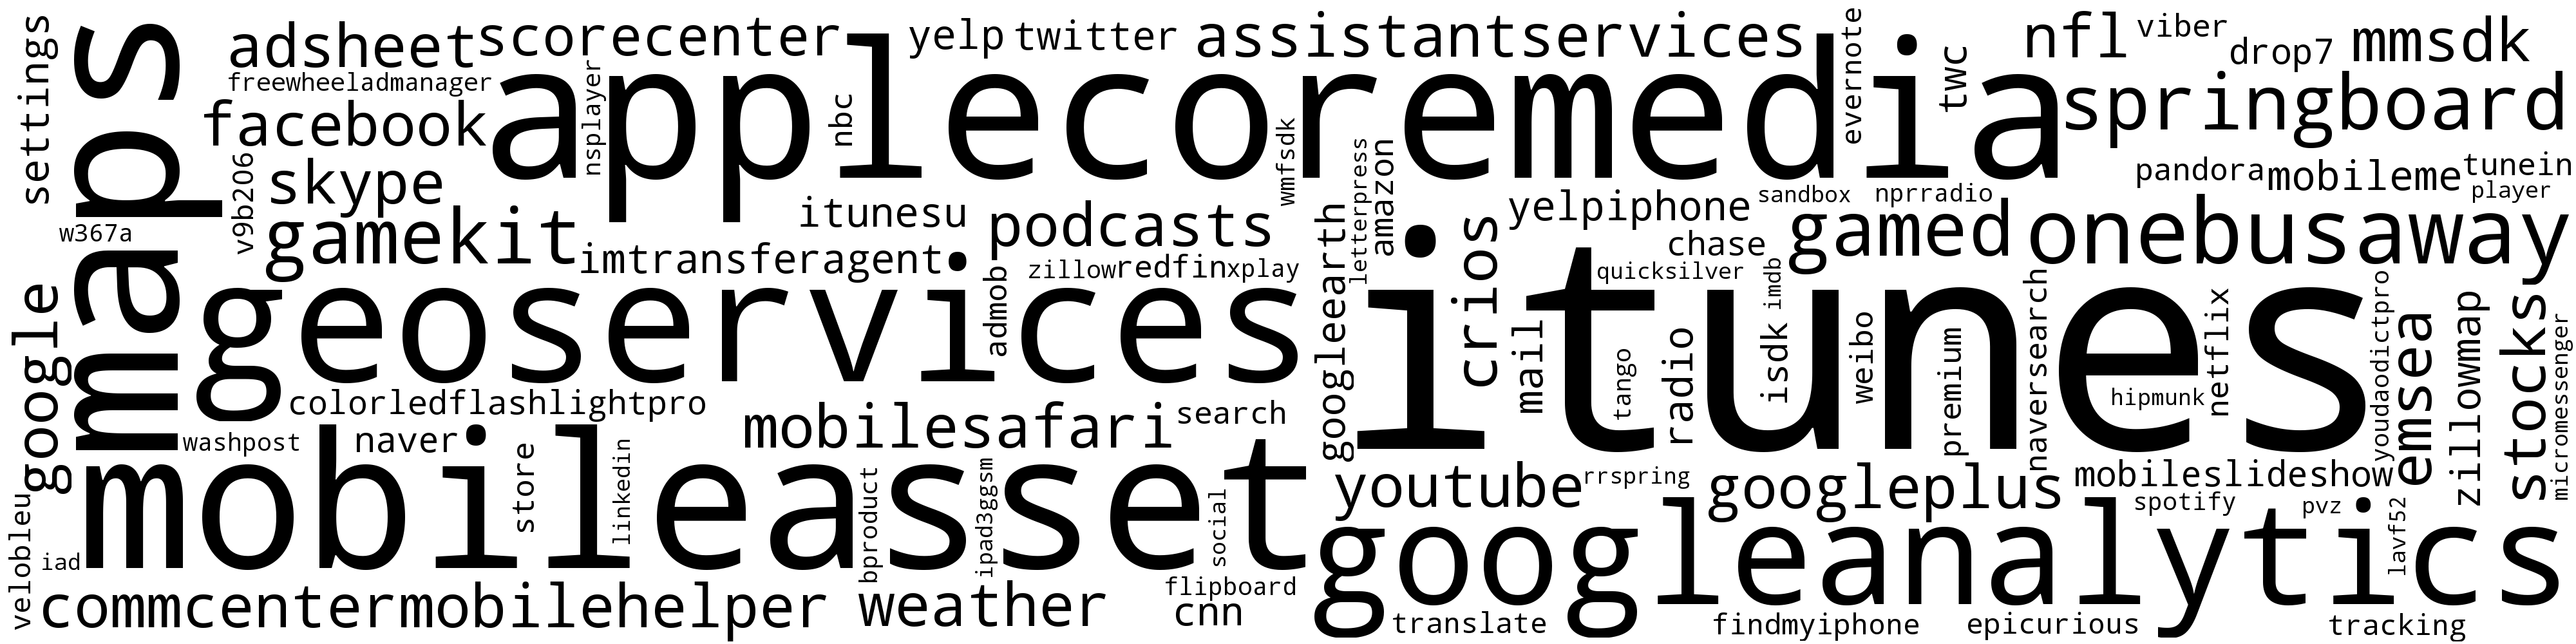
\includegraphics[width=\columnwidth]{figures/wordcloud_useragentsignature_ios_image.png}}\newline
\subfloat[Android]{\label{fig:http-wordcloud-android}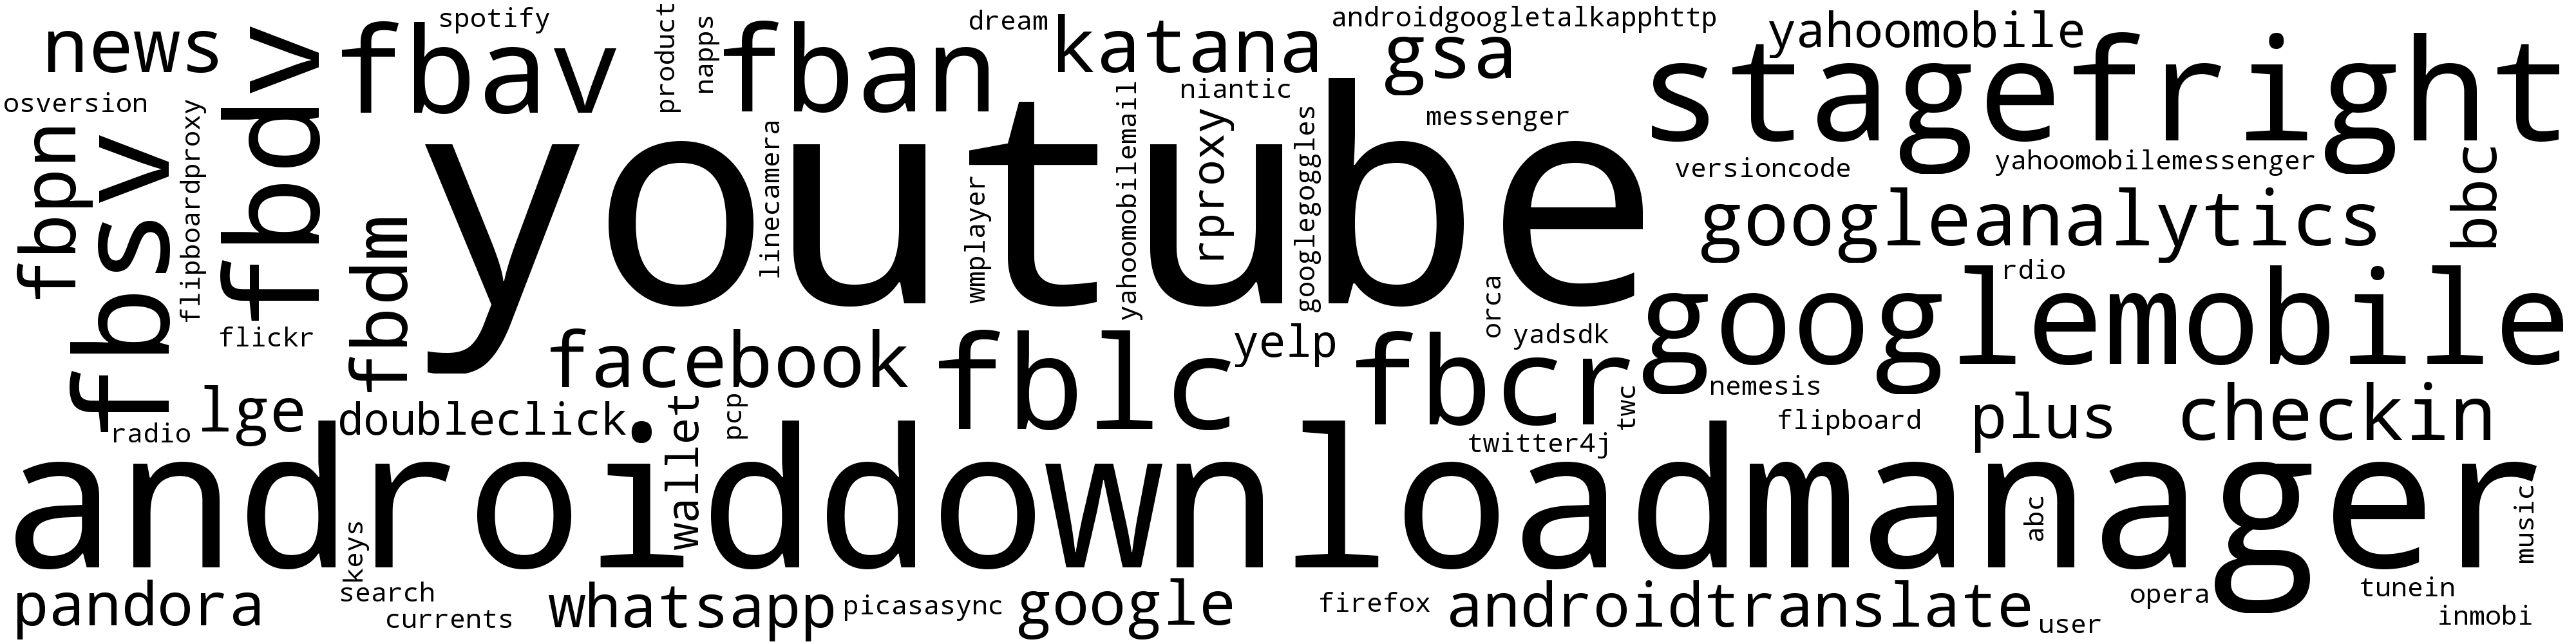
\includegraphics[width=\columnwidth]{figures/wordcloud_useragentsignature_android_image.png}}
\caption{\useragent signatures in  iOS and Android HTTP flows. \emph{The font weight represents the number of users for which a particular signature was observed}.}
\label{fig:http-wordcloud}
\end{figure}

We observe that more than 98\% of HTTP traffic from Android and iOS devices in the \mobWild dataset have a valid \useragent string; we observe a total of 1435 unique \useragent strings across Android and iOS devices. 
These \useragent strings contain an application identifier and other auxiliary information such as details of the OS, manufacturer, display resolutions, carrier, and information such as versions and compatibility with other browser engines~\cite{mozilla:useragentdetection}. 
We use regular expression to extract the tokens containing the application information and we then cluster these tokens using edit distance between individual tokens and number of matching tokens\footnote{We plan to release this code along with \platname package.}.
At the end of this process we were able to identify 361 unique application signatures.

In \fref{fig:http-wordcloud} we present a \emph{word cloud} of the signatures we were able to extract from \useragent field; the text size of the signature represents the number of users for which the signature was observed.
We clearly observe that iTunes is the most popular service for iOS devices, primarily because iTunes is the only official source for application downloads for iOS devices. 
Similarly, we observe that YouTube is one of the popular applications for the Android devices in our dataset.
Despite the usefulness of the \useragent, we observe that relying only on the \useragent is not sufficient to classify traffic from Android devices. 
For example, we were able to classify on 23.9\% of traffic from one Android device that tunneled 9.6~GB of traffic; we observe similar behavior for other Android users.
This is in complete contrast to the more than 90\% of traffic that we were able to identify on the iOS devices. 
A closer observation showed us that this difference is because of the techniques used by Android and iOS devices to download media content. 

\begin{figure}
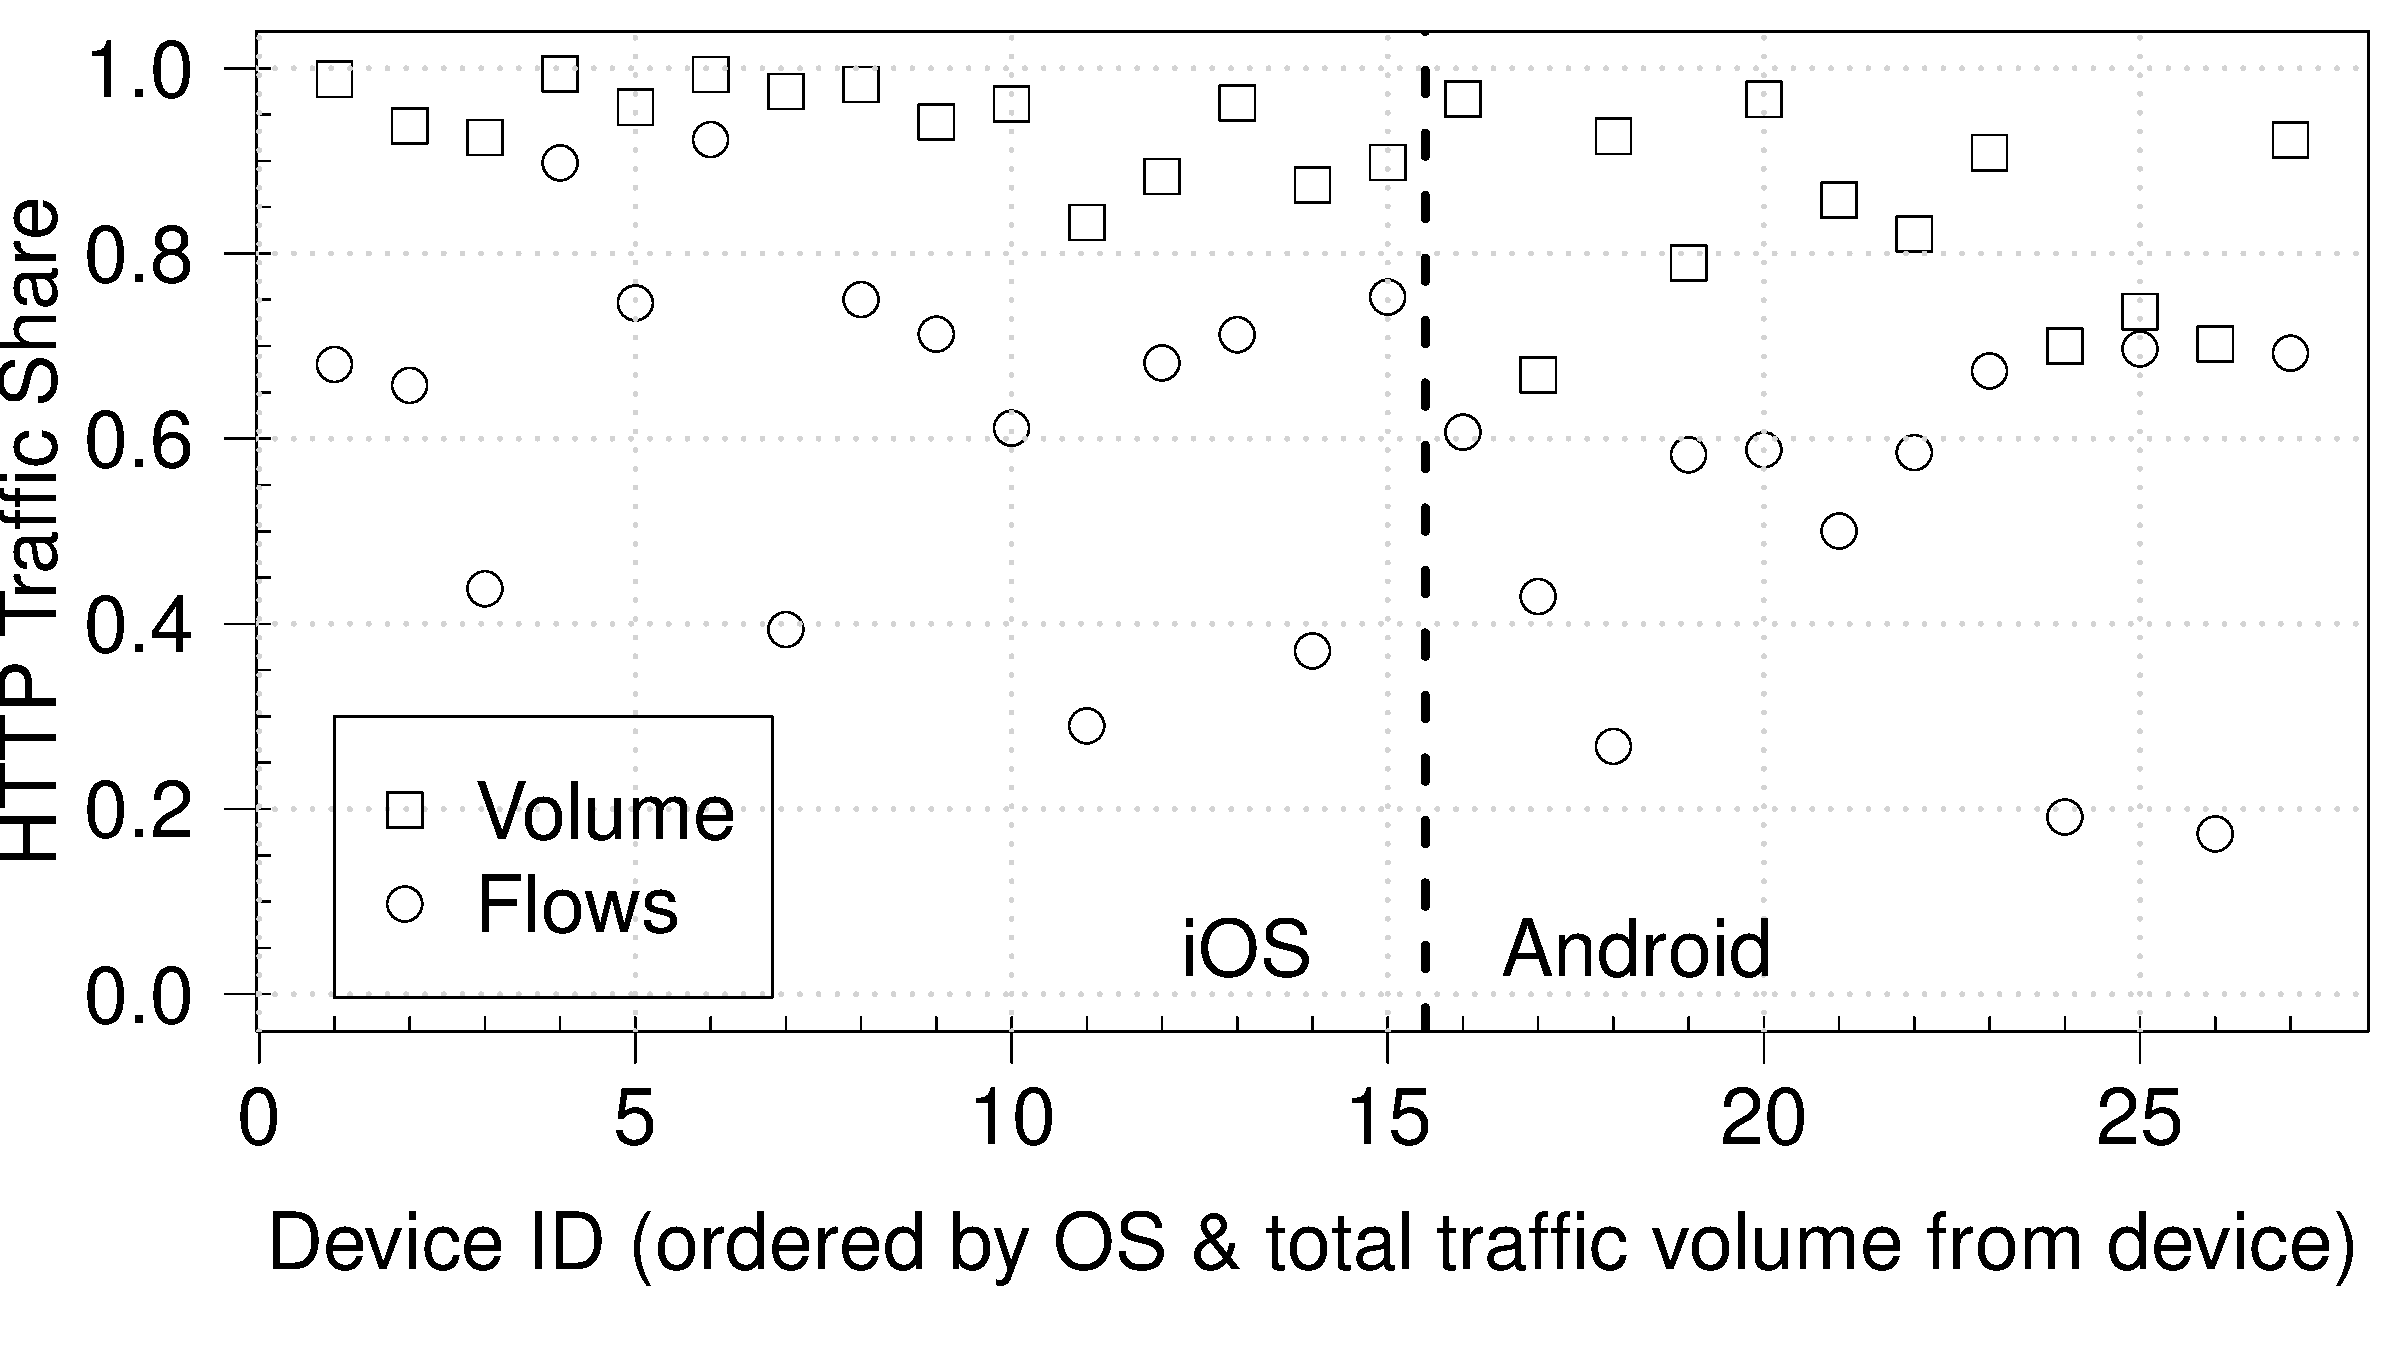
\includegraphics[width=\columnwidth]{plots/appusage_someappservicesig_traffic.pdf}
\caption{HTTP traffic classified using \useragent or \httphost field provided by popular media services in the HTTP header. \emph{\tbd{AR: Add traffic from browsers because this does not include traffic from flows that have UA of browsers -- this is the reason why the number of flows is so low.}.}}
\label{fig:http-classification-app-user-agent-host}
\end{figure}

The iOS devices rely on AppleCoreMedia service~\cite{apple:coremedia} to download media content.
We therefore observed the signature of AppleCoreMedia in more than 98.45\% of the content downloaded from the YouTube servers (which we identify based on the \httphost field in the \httpget requests). 
However, despite the availability of libraries such as Stagefright\cite{android:stagefright} to download media content, we observed that a majority of media content is downloaded without any application or OS service signature.
\tbd{verify for Android 4.2 or is this behavior specific to 4.0 and 4.1}.
Indeed, on closer observation of the traffic we observed that a large fraction of the unclassified traffic was due to media sites which we could identify based on the \httphost field in the HTTP GET request. 
We therefore used the \httphost field to identify the applications for the flows that were not classified using the \useragent field. 
In \fref{fig:http-classification-app-user-agent-host} we present the HTTP traffic share that we could classify using the \useragent field followed by the \httphost field for that could not be classified using the \useragent.
We do not use the \httphost field on its own because applications such as Facebook allow users to access websites from within their application. 

\subsubsection{Classification of SSL Traffic.}

Unlike HTTP flows, SSL flows provide limited information that can be used to identify the applications. 
We now show how we used the \sslservername and the DNS queries to classify SSL traffic. 

\begin{figure}[t]
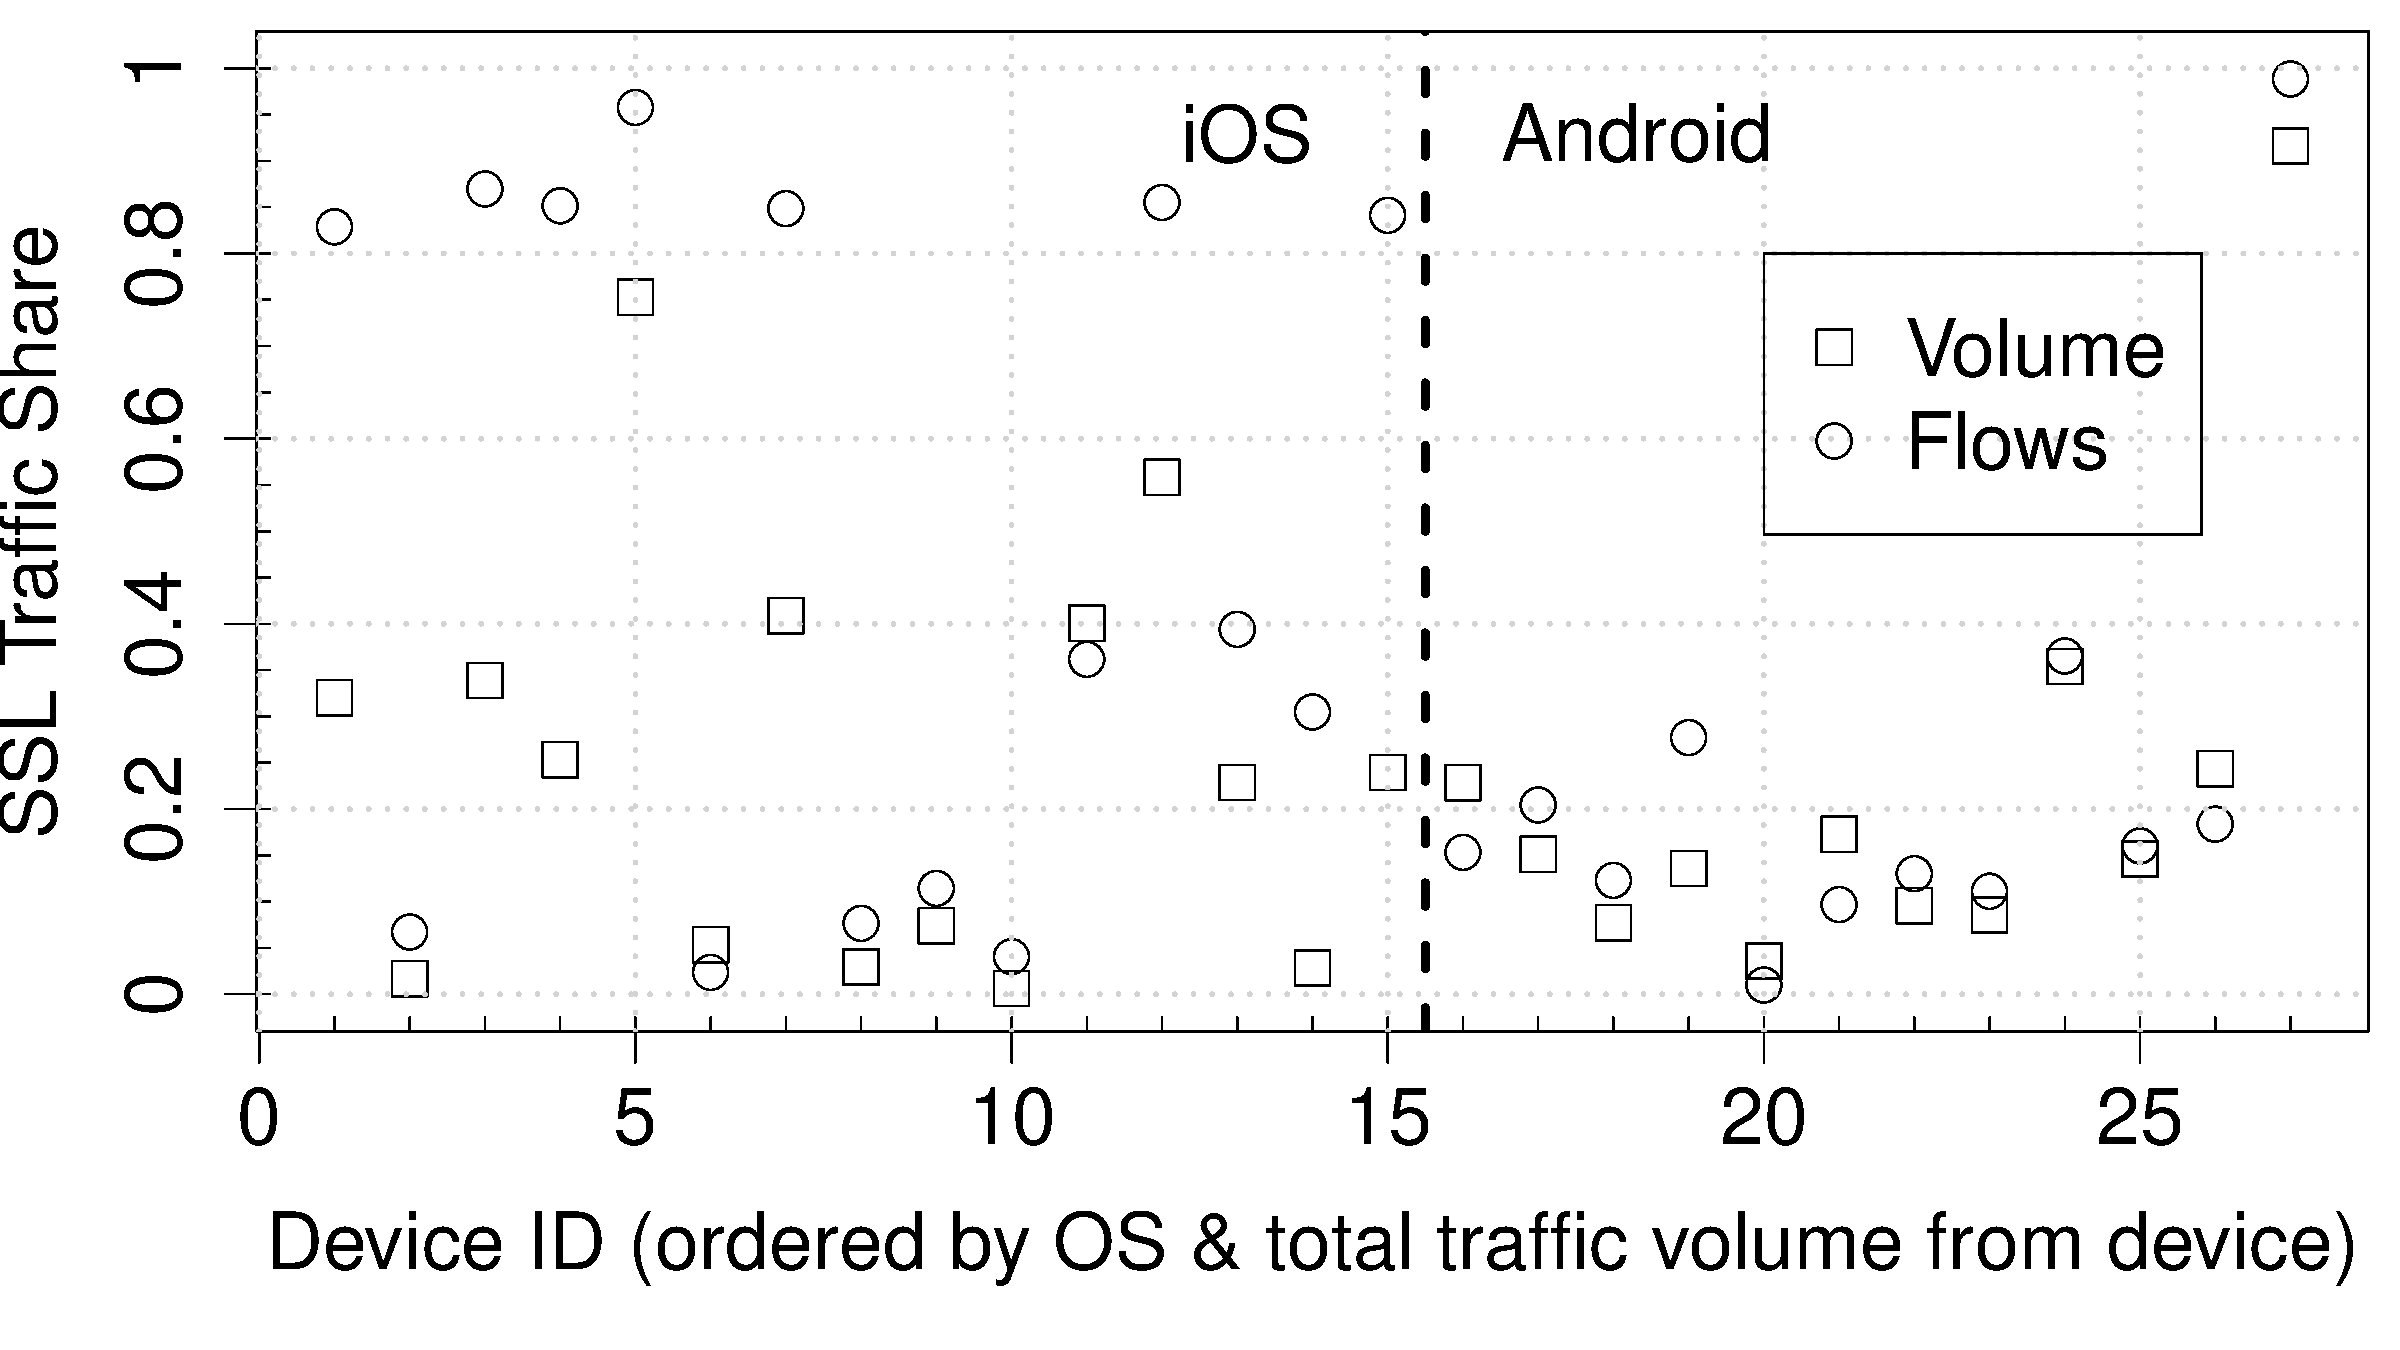
\includegraphics[width=\columnwidth]{plots/sslanalysis_someservername_traffic.pdf}
\caption{SSL flows classified using the \sslservername in the flows.}
\label{fig:ssl-classification-servername}
\end{figure}
\begin{figure}[t]
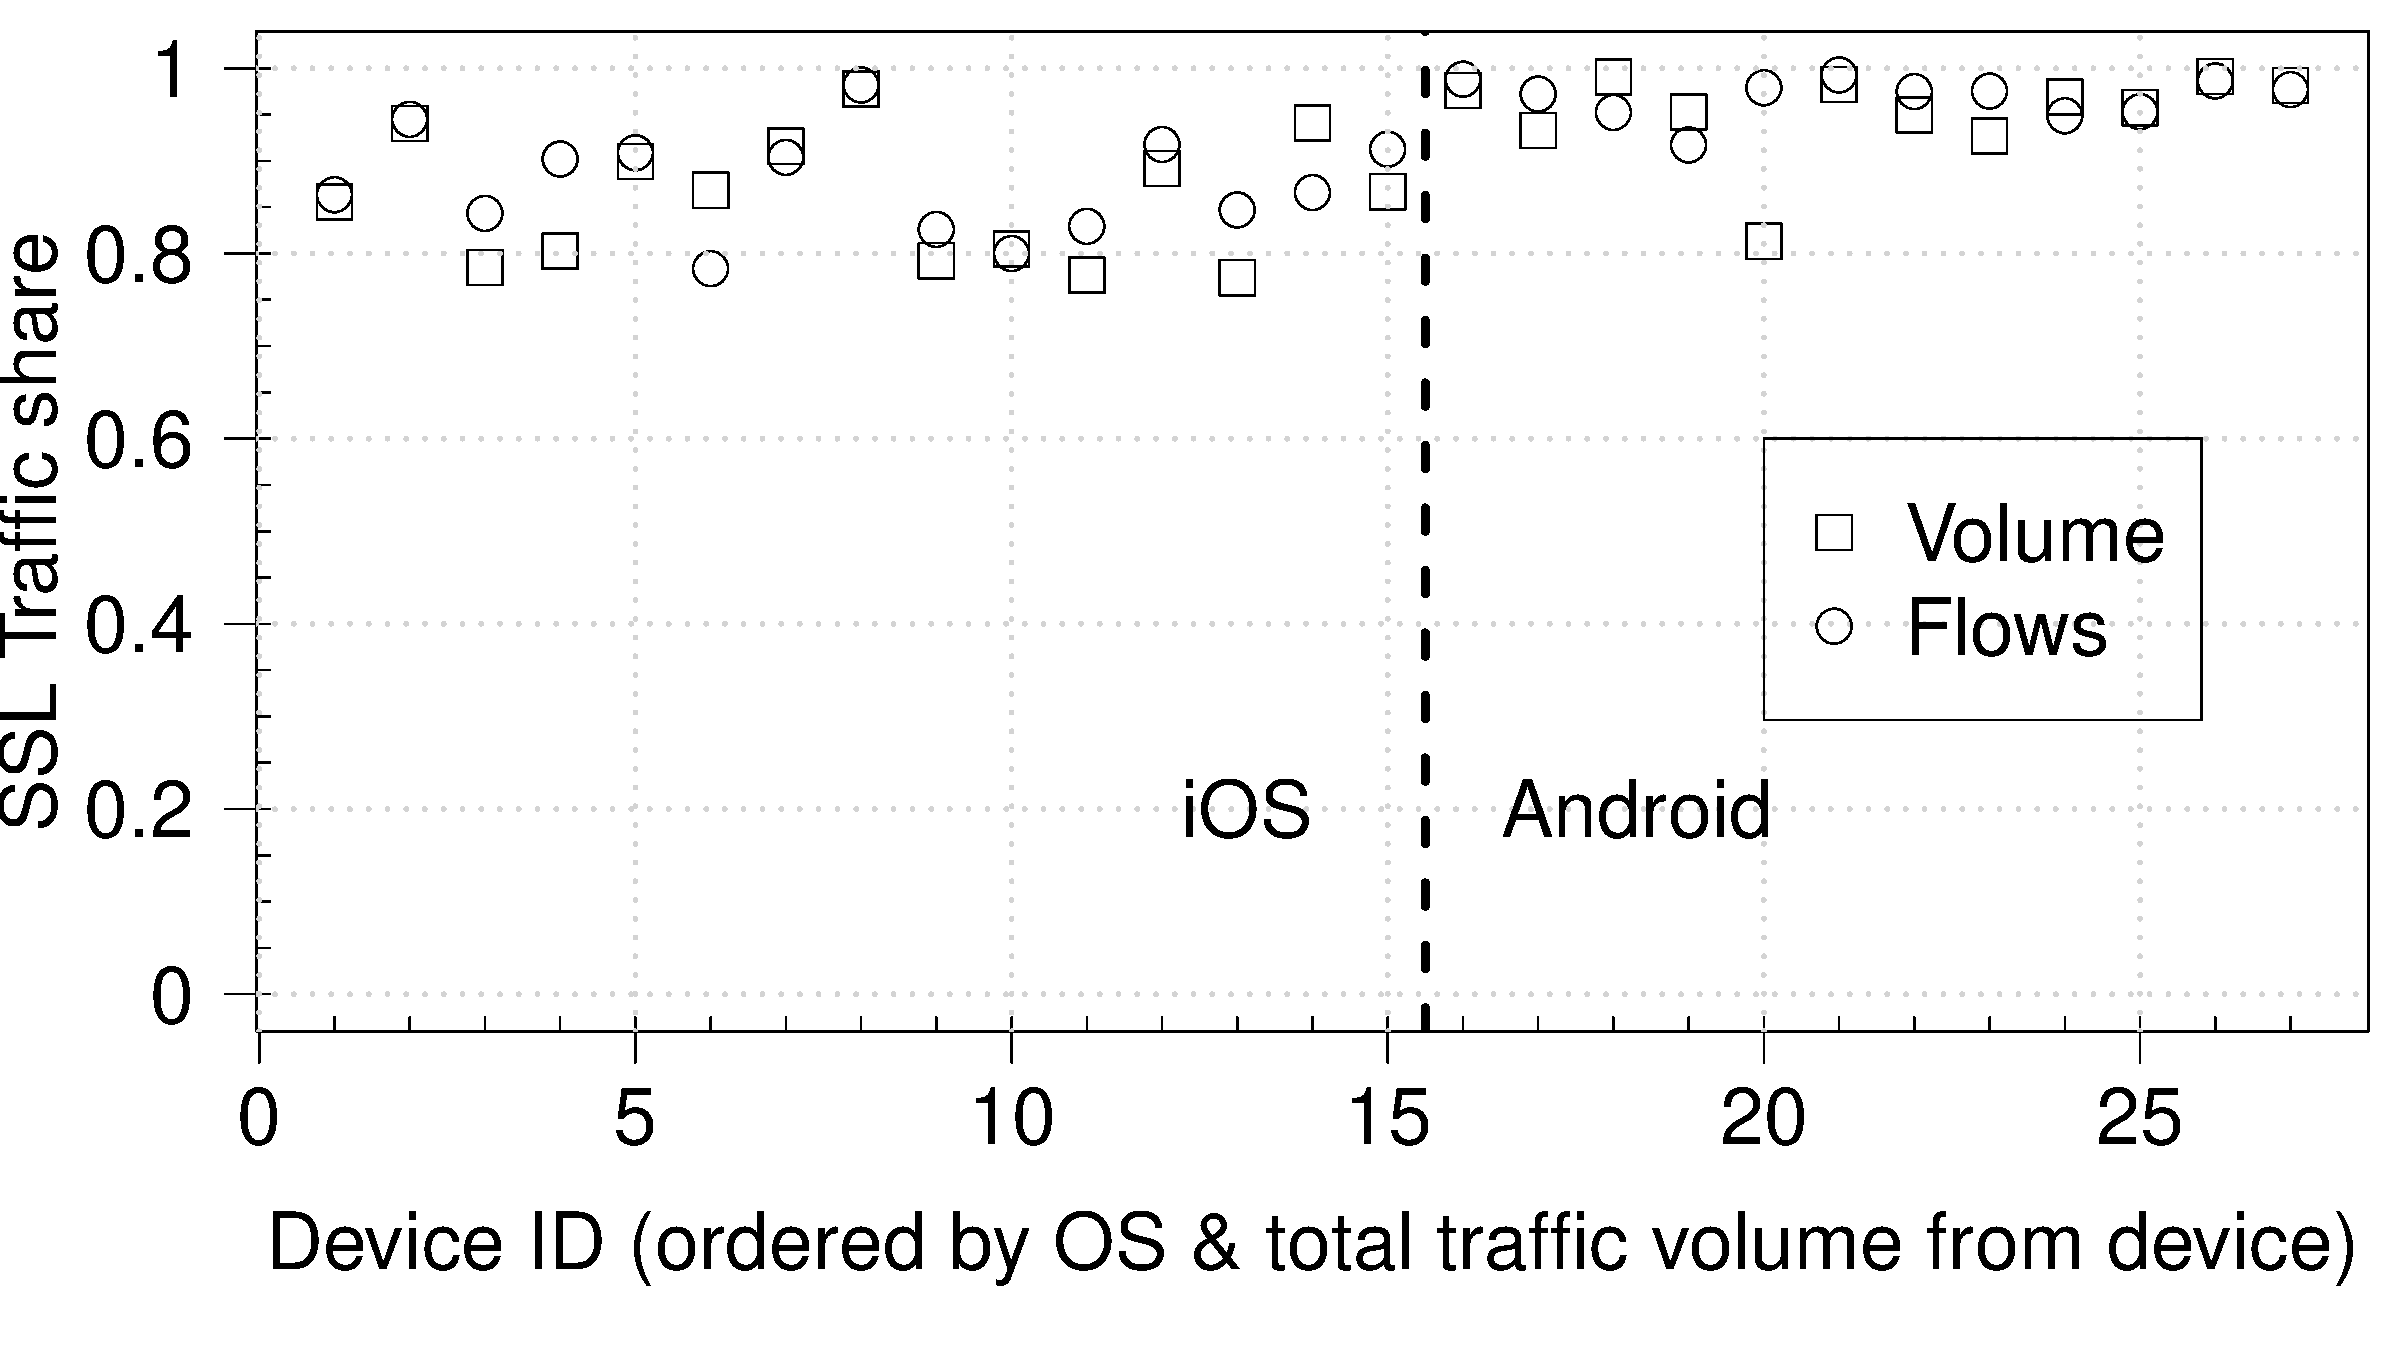
\includegraphics[width=\columnwidth]{plots/sslanalysis_samedns_traffic.pdf}
\caption{SSL traffic share where the most recent DNS response contained the IP address of the SSL flow in the first position.}
\label{fig:ssl-classification-app-service}
\end{figure}


In \fref{fig:ssl-classification-servername} we observe that relying on the \sslservername is not sufficient to classify the traffic. 
We observe a huge disparity in the fraction of traffic that can be classified using this technique.
Along with the \sslservername, the common name field of the certificate can be used to identify the traffic. 
However, the use of CDNs and the use of regular expression to support a large set of hostnames gives a us a result similar to that observed in \fref{fig:ssl-classification-servername}.

\tbd{The plot can be removed and the discussion with CN field can be merged to indicate relying on certificates and server-names on their own is not sufficient}
% \begin{figure}
% 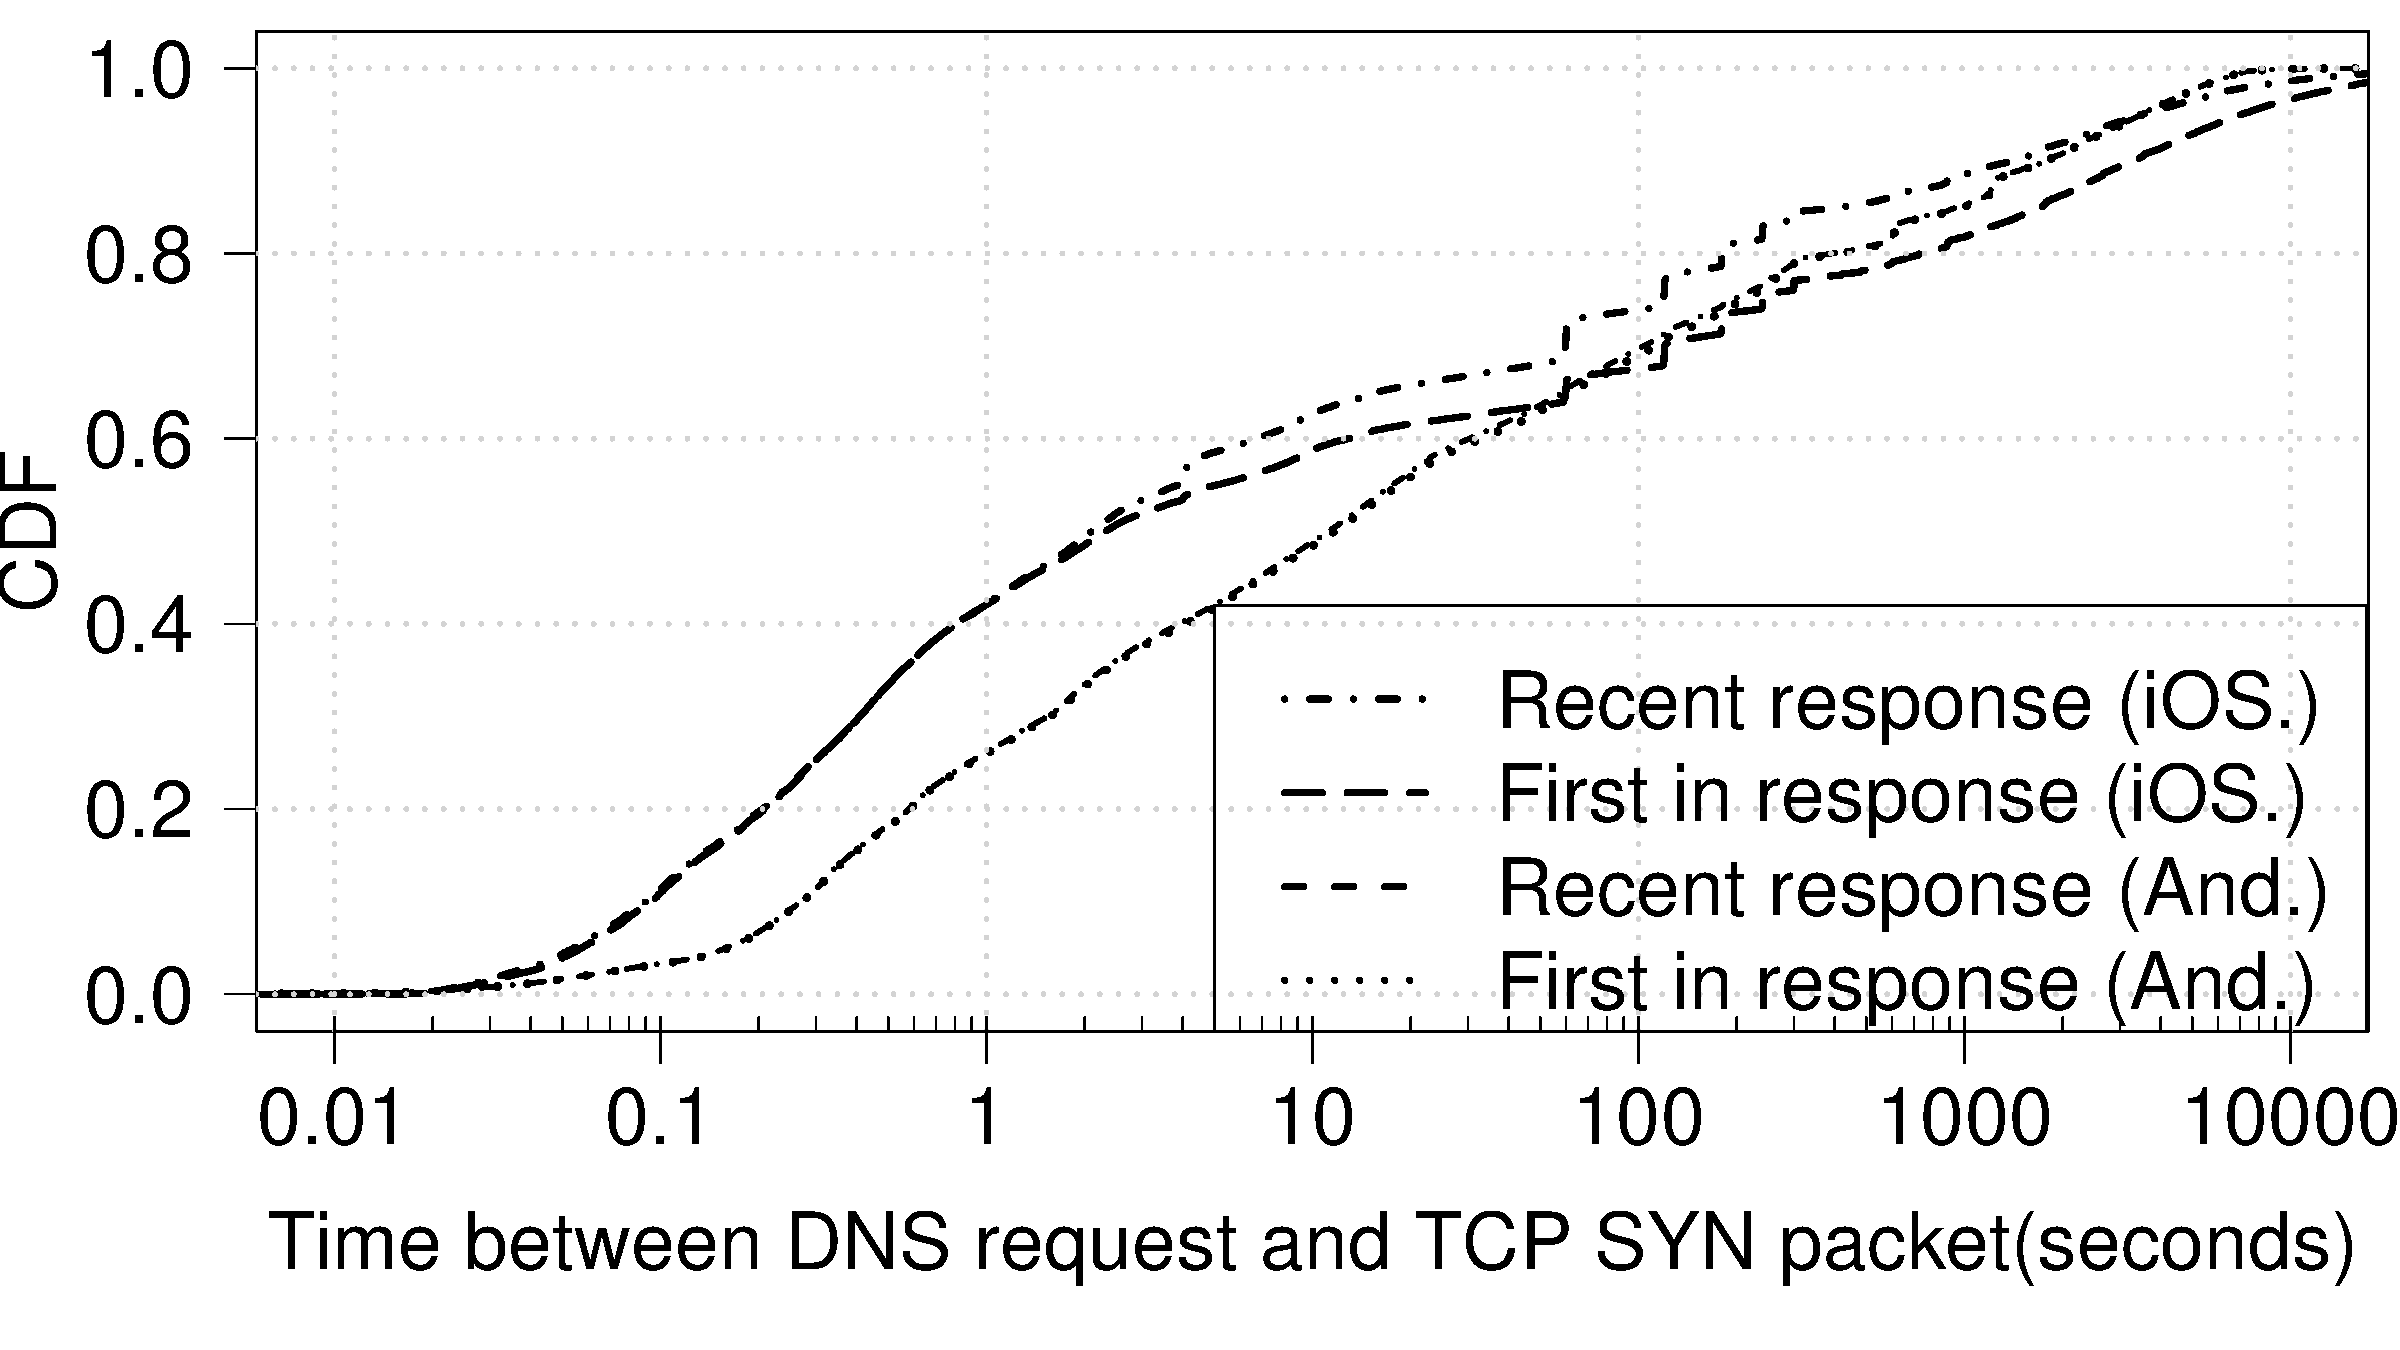
\includegraphics[width=\columnwidth]{plots/sslanalysis_dns_timediff_distrib.pdf}
% \caption{Distribution of the time between DNS response that contained the IP address of the SSL server and the SYN from the SSL flows. 
% \emph{The lack of difference in the curves for Android devices implies that the first entry in the most recent DNS response contained the IP address of the SSL flow.\tbd{rename xlab to DNS response.}}}
% \label{fig:ssl-dns-first-recent-distrib}
% \end{figure}

% To analyze the impact of the ambiguity, in \fref{fig:ssl-dns-first-recent-distrib} we plot the distribution of the time between the DNS response that contained the IP address and SYN packet from the SSL flow. 
% For this plot, we consider two types of DNS responses: the most recent DNS response that contain the IP address in the SSL flows, and the most recent DNS response that contained the IP address as the first entry in the DNS response. 
% We observe that for Android flows we do not observe a difference in the curves for the distribution, implying that the first entry in the most recent DNS response contained the IP address of the SSL flow.
% However, for iOS devices we observe a difference in the distribution when the time difference between the SYN and DNS response is larger than three seconds. 
% This difference creates an ambiguity which can be aggravated by caching of name resolution by the applications. 

We use the DNS flows that passed through \platname to further classify the SSL flows, a technique similar to DN-Hunter~\cite{bermudez:dnhunter}.
DN-Hunter relies on the most recent FQDN that corresponds to the IP address, however in our controlled experiments we observe Android and iOS devices prefer the the first entry in DNS response while resolving \emph{hostnames}.
Popular webservices such as google are known to use the same pool of IP addresses for various applications, for example the IP for gmail may also be used for search. 
In \fref{fig:ssl-classification-app-service} we present the fraction of SSL traffic where the most recent DNS response contained the IP address of the SSL flow in the first position. 
We observe that for the majority of SSL traffic by volume and flows can be classified by using the DNS responses. 

In summary, we use \platname to perform controlled experiments and in the wild measurements to characterize mobile Internet traffic. 
We use Bro to analyze the data and build on the output of bro to further classify HTTP flows and SSL flows to identify the source of the traffic. 
We now present the results of our experiments and measurements study. 


%%% Local Variables: 
%%% mode: latex
%%% TeX-master: "main"
%%% End: 

% We used Bro~\cite{bro} to analyze the traffic the passed through our \platname servers.
% In \fref{tab:summaryIOSAndroidTraffic} we summarize \mobWild based on the classification performed using Bro~\cite{bro}.
% Bro classifies IP flows using the protocol field in the IP header.
% We use this classification to label flows as either TCP, UDP, or \emph{other}; flows that are neither TCP nor UDP are classified as \emph{other}. 
% Bro further uses the well defined port numbers to identify the services that use TCP.
% We use this classification to label flows as either HTTP, SSL (which includes HTTPS, IMAP, etc.) or \emph{other} flows; TCP flows that are not classified as either HTTP or SSL are classified as \emph{other}.
% In \fref{tab:summaryIOSAndroidTraffic}, we observe that more than 90\% of the traffic in our dataset is either HTTP or SSL. 
% We also observe that the share of HTTP volume over \wifi and cellular are significantly different. 
% As detailed in \fref{sec:.}, this difference is primarily due to the use of \wifi to transfer media content.
% We also observe the share of SSL traffic over cellular networks is considerably larger compared to \wifi networks.
% This increase is a result of the reduced share of media traffic and the use of email and for social networking applications that rely on SSL.
% We detail the HTTP and SSL traffic from iOS and Android devices in \fref{sec:}

% We focus our application classification on TCP because TCP is responsible for than 90\% of the traffic volume in our dataset (see~\fref{tab:summaryIOSAndroidTraffic}).
% \begin{figure}
% 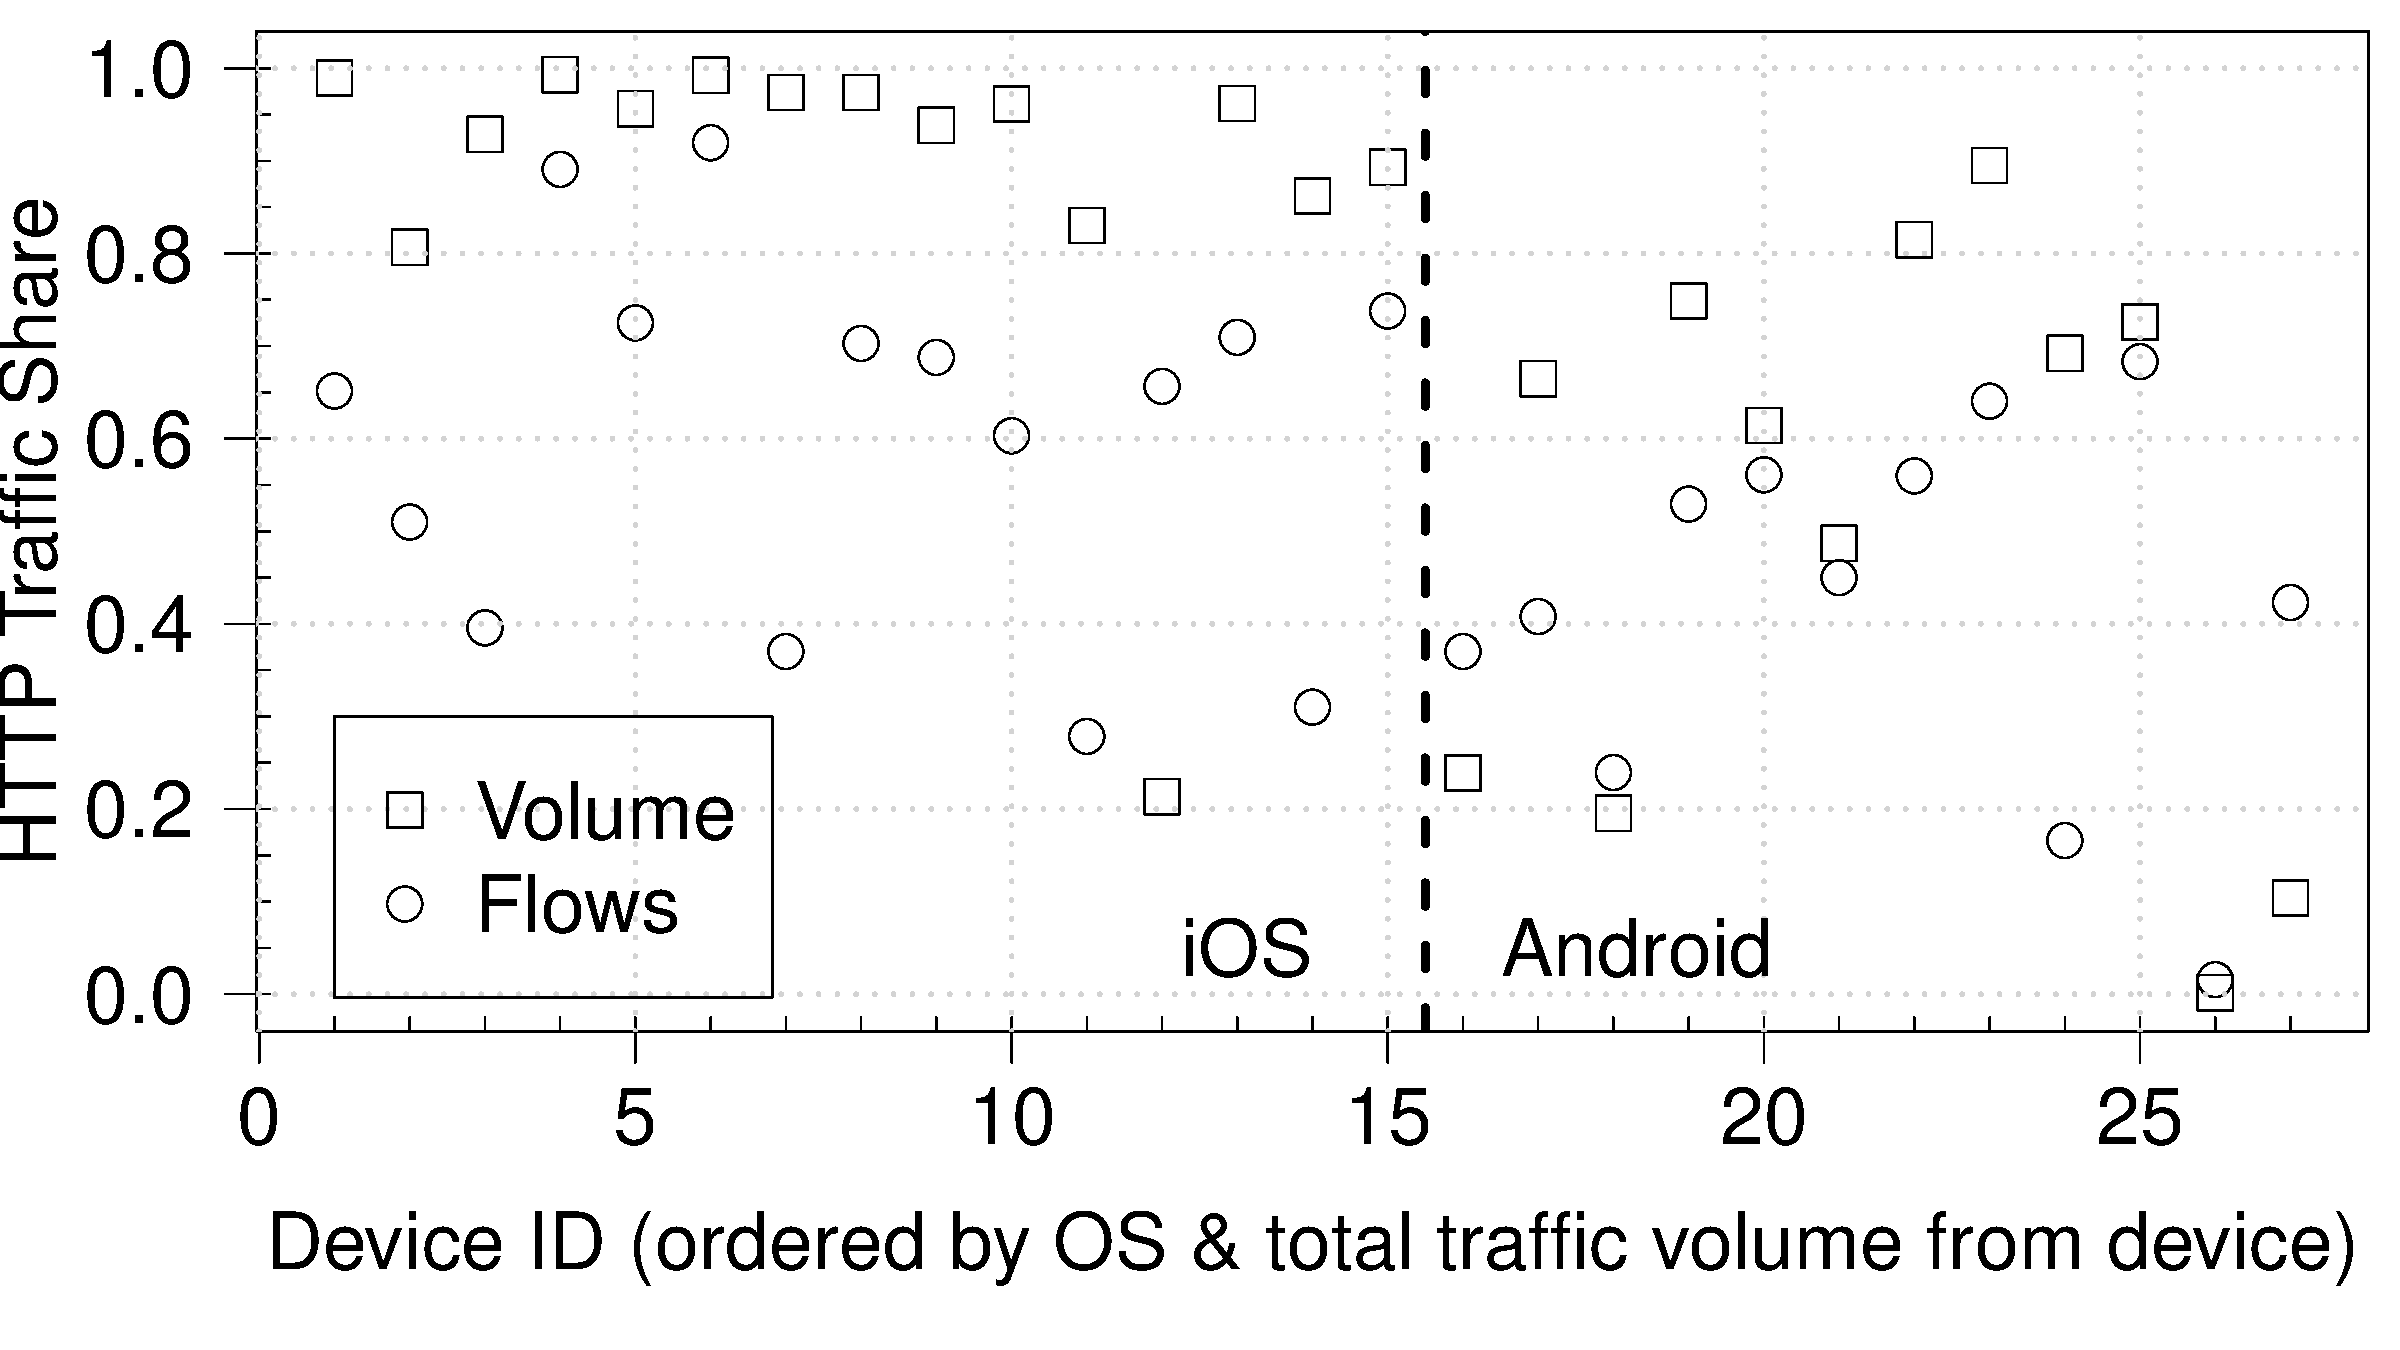
\includegraphics[width=\columnwidth]{plots/appusage_someappsig_traffic.pdf}
% \caption{HTTP traffic with a \useragent field containing an identifier of an application (other than Web-browser) or an OS service. 
% \emph{A smaller share of Android HTTP traffic can be classified using User-Agents because Android applications are not limited to underlying OS media services such as AppleCoreMedia.}}
% \label{fig:http-classification-app-user-agent}
% \end{figure}

% In \fref{fig:http-classification-app-user-agent} we plot the fraction of HTTP traffic for we were able to identify an application signature; the devices are ordered according to the operating system, and for each operating system we further order the devices according to the total traffic from the device that flowed through \platname. 
% We observe that a significantly larger fraction of traffic from iOS device can be mapped to an application in comparison to the traffic from Android devices. 
% For example, while more than 80\% of HTTP traffic from iOS devices contain an application or OS service signature in the \useragent field, only 23.9\% and 19.5\% from Android devices with id 16 and 18 contained useful signatures in the \useragent field.
% On further inspection we observe that this difference is because of the techniques used by Android and iOS application to download audio and video content. 
